\documentclass[a4paper,12pt]{article} 
\usepackage[utf8x]{inputenc}
\usepackage[french]{babel}
\usepackage{mathtools}
\usepackage{amsmath, amssymb, amsfonts}
\usepackage{textcomp}
\usepackage[nointegrals]{wasysym}			% Collection de symboles mathématiques
\usepackage{ifthen}
\usepackage{tabularx}	 				% Gestion avancée des tableaux
\usepackage{longtable}		
%\usepackage{cleveref}

\usepackage{mathrsfs}

\usepackage{enumitem}
\usepackage{wrapfig}
%\usepackage[squaren]{SIunits}
%\usepackage[T1]{fontenc}				% Indispendable, présent dans tous les codes exemples
\usepackage[linkcolor=Indigo, colorlinks=true, citecolor=DarkSlateBlue, urlcolor=MidnightBlue]{hyperref} 	% Hyper ref
\usepackage{listings}					% Pour citer du code
\usepackage[justification=centering]{caption}
\usepackage{sistyle} 
\usepackage{numprint}
\usepackage{wrapfig}
\usepackage{cite}	
\usepackage{url} 					% Pour citer les sites internet dans la
%\usepackage{cleveref}4
\usepackage{setspace}
\usepackage{graphicx}		 			% Inclusion des figures
\graphicspath{{./pic/}, {../figures/full_69_rapport/}}

\newcommand{\bepar}[1]{
	\left( #1 \right)  
}

\setlength{\parindent}{0pt}

\usepackage[svgnames]{xcolor}			%https://www.latextemplates.com/svgnames-colors

\title{\large{Licences SESI \& SESI/PEIP -- Semestre 1}}%%%%%%%%%%%%%%%%%%%%
\date{\large{18 Octobre 2018}}

%%%%%%%%%%%%%%%%%%%%
%%% Couleurs %%%
\xdefinecolor{brick}{named}{DarkRed}
\xdefinecolor{navy}{named}{Navy}
\xdefinecolor{midblue}{named}{MidnightBlue}
\xdefinecolor{dsb}{named}{DarkSlateGray}
\xdefinecolor{dgreen}{named}{DarkGreen}

%%% 	Raccourcis 	%%%
\newcommand{\keps}{$k-\varepsilon$}
\newcommand\bk{\color{black}}
\newcommand\brick{\color{brick}}
\newcommand\navy{\color{navy}}
\newcommand\midblue{\color{midblue}}
\newcommand\dsb{\color{dsb}}
\newcommand{\dgreen}{\color{dgreen}}
\newcommand\red{\color{red}}

%%%%%%%% Cigles
\newcommand{\rap}{par rapport}
\newcommand{\cad}{c'est-à-dire}
\newcommand{\vav}{vis-à-vis}


%\usepackage{fancyhdr}
%\pagestyle{fancy}
%\fancyhead[RO]{\thepage}
%\fancyhead[RO]{}
%\lhead{
%\rhead{}
%\rhead{\markright}
\usepackage{geometry}
\geometry{hmargin=2.4cm, vmargin=3cm}

\usepackage{fancyhdr}
 
\pagestyle{fancy}
\fancyhf{}
\fancyhead[LE,RO]{Année 2018-2019}
\fancyhead[RE,LO]{ Université de Lille -- Faculté des Sciences et Technologies}

\begin{document}
\begin{center}
	\large{\textbf{Initiation à la Mécanique des Fluides}} \\[1mm]
	\textit{Exercices complémentaires.}
\end{center}

\textbf{\textit{Notez}} : 
	\begin{itemize}[leftmargin=1.4cm]
		\item[1-] \textit{Ces exercices ont pour but de tester votre compréhension du TD 1 essentiellement. Il est donc indispensable d'avoir au préalable compris ce TD.}
 		\item[2-] \textit{ Ces exercices ne sont que des propositions. Il en existe des centaines d'autres dans les bouquins.}
		\item[3-] \textit{L'exercice sur la montgolfière est assez poussé.}
\end{itemize}
\hrule
\vspace{2mm}

\brick \subsection*{TD1} \bk

\navy \subsubsection*{Équilibre de trois liquides non miscibles (exo 1 TD)} \bk

\begin{wrapfigure}{R}{0.24\textwidth}
	\vspace{-1cm}
	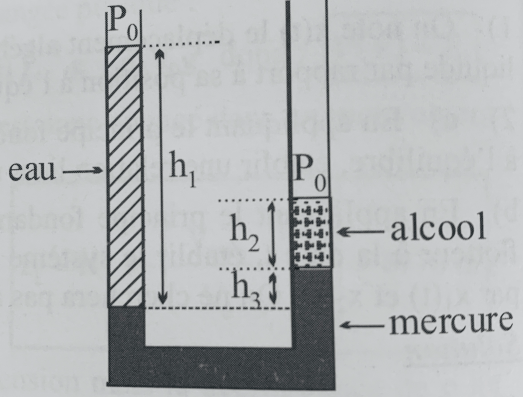
\includegraphics[scale=0.27]{tube.png}
\end{wrapfigure}

Un système 	de trois liquides non miscibles entre eux (eau, mercure, alcool) est en équilibre dans un tube en U ouvert à l'air libre à ses deux extrémités. \\[2mm]
On note $P_0$ la pression atmosphérique, $h_1$ et $h_2$, les hauteurs respectives d'eau. d'alcool, $h_3$ la dénivellation entre les niveaux de mercure dans les 2 branches, $\rho_1$, $\rho_2$ et $\rho_3$ les masses volumiques l'eau, de l'alcool et du mercure. \\

Exprimer $\rho_2$ en fonction de $\rho_1$, $\rho_3$, $h_1$, $h_2$ et $h_3$\\
A.N. : $\rho_1 = 10^3$ kg.m$^{-3}$; $\rho_3 = 1\pnt36 \times 10^4$ kg.m$^{-3}$; $h_1=0\pnt8$ m, $h_2=0\pnt15$ m et $h_3=0\pnt05$ m

\navy \subsubsection*{Poussée sur deux barrages plans (exo 9 TD)} \bk
Deux barrages de profil droit, l'un vertical et l'autre oblique incliné d'un angle $\alpha$ avec la verticale, permettent de réaliser une retenue d'eau sur une hauteur h et une largeur L.\\[2mm]
On note $P_0$ la pression atmosphérique, et $\rho_0$ la masse volumique de l'eau, considérée comme constante.\\

Déterminer dans les deux cas les composantes $F_x$ et $F_z$ de la résultante $\vec{F}$ des forces de pression qu'exerce l'eau sur la surface S du barrage.

\begin{figure}[!ht]
\centering
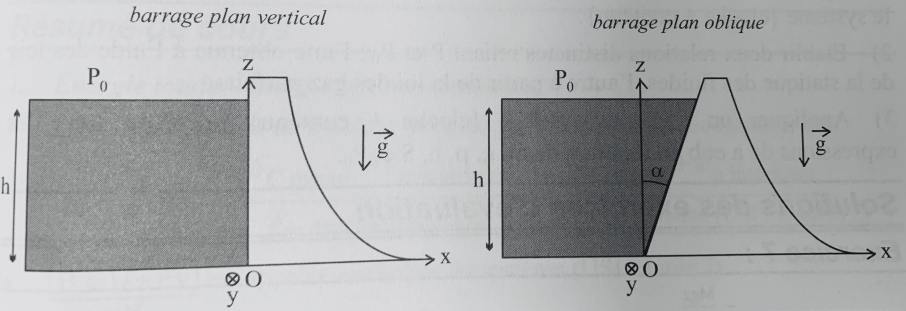
\includegraphics[scale=0.4]{barr.png}
\end{figure}

\pagebreak

\navy \subsubsection*{Baromètre à deux liquides exo 1,2} \bk
On désire comparer les performances d'un baromètre classique à mercure et d'un baromètre à deux liquides, mercure et glycérine. Ce dernier dispositif est constitué d'une cuve à mercure et d'un tube barométrique de section $S_2$ comportement un renflement de section $S_1$.\\
On note $\rho$ la masse volumique du mercure et $\mu$ celle de la glycérine.\\

Pour une valeur $P_0$ de la pression atmosphérique, l'équilibre est caractérisé par une hauteur $h$ de mercure dans le baromètre classique, et par une hauteur $h_1$ de mercure surmontée par une hauteur $h_2$ de glycérine dans la baromètre à deux liquides (voir figures ci-dessus, parties gauches).\\
Lorsque la pression atmosphérique varie et prend la valeur de $P = P_0 + \Delta P$, la hauteur de mercure dans le baromètre classique varie de $\Delta h$, et les altitudes des niveaux supérieurs de mercure et de glycérine dans le baromètre à deux liquides varient de $\Delta z_1$ et $\Delta z_2$ (voir parties droites), l'axe Oz désignant la verticale ascendante.\\
On néglige la variation du niveau de mercure dans les cuves, et on suppose que la surface mercure-glycérine est toujours située dans la zone de renflement.
\begin{figure}[!ht]
\centering
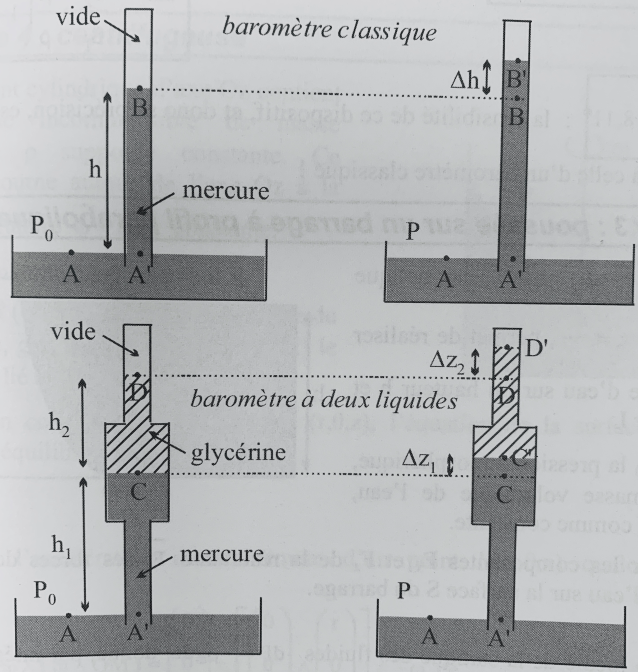
\includegraphics[scale=0.35]{barometre.png}
\end{figure}

\begin{itemize}[leftmargin=1.4cm]
	\item[1)] Quelques relations :
	\begin{itemize}
		\item[a)] Donner la relation liant $\Delta P$ et $\Delta h$
		\item[b)] Donner la relation liant $\Delta z_1$ et $\Delta z_2$ exprimant l'incompressibilité (conservation du volume) de la glycérine.
		\item[c)] Trouver la relation entre $\Delta P$, $\Delta z_1$ et $\Delta z_2$. En déduire le rapport des surélévations $\Delta z_2$/$\Delta h$ en fonction $\rho$, $\mu$, $S_1$ et $S_2$. 
	\end{itemize} 

	\item[2)] A.N.: $S_1 = 5$ cm$^2$;  $S_2 = 0\pnt25$ cm$^2$; $\rho = 13600$ kg.m$^{-3}$; $\mu=1050$ kg.m$^{-3}$.\\[2mm]
	Interpréter ce résultat. Quel est l'intérêt de ce dispositif ?
	
\end{itemize}

\navy \subsubsection*{Ascension d'une montgolfière} \bk
Un aérostat (autre nom de la montgolfière) est constitué d'une enveloppe souple de volume maximale $V_{\text{max}}$ gonflée à l'hélium. L'enveloppe, la nacelle, les accessoires et les passagers ont une masse totale m.\\
L'équilibre mécanique entre l'hélium et l'air extérieur est assuré par l'élasticité de l'enveloppe tant que $V<V_{\text{max}}$, et par une soupape située à son sommet lorsque $V=V_{\text{max}}$.\\[2mm]
L'aérostat évoluant dans la troposphère\footnote{\url{https://en.wikipedia.org/wiki/Troposphere}}, la température de l'air peut être modélisée par (H constante) $$T(z) = T_0 \bepar{1 - \frac{z}{H}} $$
On aura la température à l'intérieur du ballon $T_{\text{int}}$ égale à la température de l'air $T(z)$ à toute altitude z, de même pour les pressions à l'intérieur du ballon et de l'air\footnote{On parlera de système respectivement à l'équilibre thermique et à l'équilibre mécanique}.\\

On étudiera l'aérostat défini par le système \{masse m (nacelle) + Hélium \}. Son mouvement est \textbf{uniquement} vertical selon l'axe Oz ascendant d'origine O située au niveau du sol ($z=0$).\\

\begin{figure}[!ht]
\centering
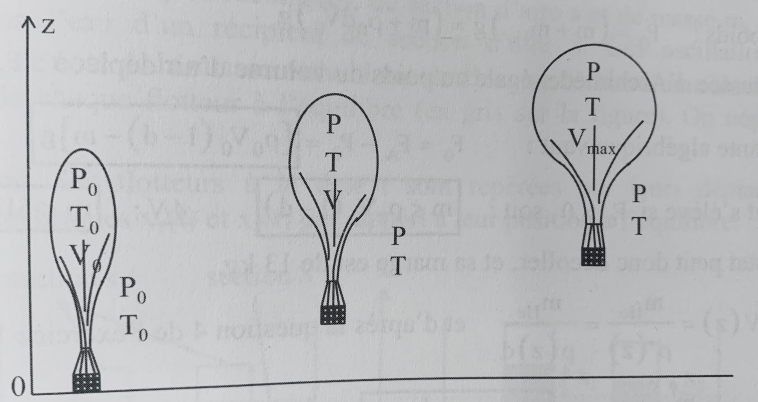
\includegraphics[scale=0.35]{mongol.png}
\end{figure}

\paragraph*{\brick Questions préliminaires : \bk}
\begin{itemize}[leftmargin=1cm]
	\item[I.1] Écire la loi des gaz parfaits en faisant apparaître la masse volumique du gaz $\rho$, $R$ la constante des gaz parfait ainsi que la masse molaire moléculaire du gaz $M$, sa pression et sa température.
	\item[I.2] Par analyse dimensionnelle, qu'elle est la dimension de $R$ ? On rappelle que la masse molaire moléculaire est donnée par $$ M = \frac{n}{m}$$ n étant le nombre de mole et m la masse du gaz.
	\item[I.3)] Calculer la masse volumique de l'air au sol $\rho_0$, sachant que $M_{\text{air}} = 29$ g.mol$^{-1}$, $T_0 = 293$ K et $P_0 = 10^5$ Pa.

	\item[I.4] À partir de calculs similaires à ceux effectués exo 3 q.3 démontrer les égalités suivantes :

	 $$ P(z) = P_0 \bepar{1 - \frac{z}{H}}^q$$ 
     $$\rho(z) = \rho_0 \bepar{1 - \frac{z}{H}}^{q-1}$$

Avec $$ q = \frac{MgH}{RT_0}$$
	
\end{itemize}	

\paragraph*{\brick Vif du sujet : \bk\\}
\textit{Pour les prochaines questions, on suppose que} $V<V_{\text{max}}$ \\[2mm]
On définit la densité de l'hélium  par rapport à l'air par le rapport de la masse volumique de l'hélium $\rho_{\text{He}}$ sur celle de l'air $\rho$ 
$$\delta = \frac{\rho_{\text{He}}}{\rho}$$ 

\begin{itemize}[leftmargin=1.4cm]
	\item[II.1] Écrire $\delta$ comme le rapport des masses molaires de l'hélium $M_{\text{He}}$ et de l'air $M$, puis calculer sa valeur. (Ind. utiliser les hypothèses de la note 2)
	\item[II.2] On appelle force ascensionnelle $F$ la résultante des forces extérieures s'exerçant sur l'aérostat.\\
	Exprimer sa valeur au sol, c'est-à-dire calculer $F_0 = F(z=0)$ en fonction de m, g, $\delta$, $V_0$ et $\rho_0$. À quelle condition sur m la masse de la nacelle, l'aérostat s'élève-t-il ? Pour répondre à cette question, on prendra $V_0 = 500 \text{ m}^3$. \\
	\textbf{Pour la suite on prendre m = 500 kg} \\[1mm]
	\item[II.3] En cours d'ascension (toujours $V<V_{\text{max}}$) exprimer :
	\begin{itemize}
		\item[a)] $V(z)$ en fonction de $q$ (défini question I.4) et de $(1-z/H)$.\\	On partira de la définition de la masse volumique de l'hélium $\rho_{\text{He}}(z)$ et de la définition de $\delta$.
		\item[b)] Montrer que pendant l'ascension $F(z) = F_0$. Commenter \\[3mm]
	\end{itemize}
\end{itemize}

\textit{On suppose à présent que} $V\leq V_{\text{max}}$
\begin{itemize}[leftmargin=1.4cm]
	\item[II.4] Déterminer l'altitude $z_1$ telle que $V(z) = V_{\text{max}} = 1000 \text{ m}^3$. Que se passe t- il dès lors que $z > z_1$ ? Expliquer alors le rôle de la soupape (exo 1 TD 2). \\[1mm]
	\item[II.5] Vol de "croisière"
	\begin{itemize}
		\item[a)] Exprimer F(z) en fonction de m, g, $\delta$, $V_{\text{max}}$, $\rho_0$, $\bepar{1 - z/H}$ et $q$.
		\item[b)] En déduire le plafond d'altitude $z_2$ défini par $F(z_2) = 0$
		\item[c)] Comment attérir ?
	\end{itemize}
\end{itemize}


\end{document}